%File: main.tex
\documentclass[letterpaper]{article} % DO NOT CHANGE THIS
\usepackage[submission]{aaai24}  % DO NOT CHANGE THIS
\usepackage{times}  % DO NOT CHANGE THIS
\usepackage{helvet}  % DO NOT CHANGE THIS
\usepackage{courier}  % DO NOT CHANGE THIS
\usepackage[hyphens]{url}  % DO NOT CHANGE THIS
\usepackage{graphicx} % DO NOT CHANGE THIS
\urlstyle{rm} % DO NOT CHANGE THIS
\def\UrlFont{\rm}  % DO NOT CHANGE THIS
\usepackage{natbib}  % DO NOT CHANGE THIS AND DO NOT ADD ANY OPTIONS TO IT
\usepackage{caption} % DO NOT CHANGE THIS AND DO NOT ADD ANY OPTIONS TO IT
\frenchspacing  % DO NOT CHANGE THIS
\setlength{\pdfpagewidth}{8.5in} % DO NOT CHANGE THIS
\setlength{\pdfpageheight}{11in} % DO NOT CHANGE THIS

\usepackage{algorithm}
\usepackage{algorithmic}
\usepackage{newfloat}
\usepackage{listings}
\usepackage{graphicx}
\usepackage{subcaption}

\DeclareCaptionStyle{ruled}{labelfont=normalfont,labelsep=colon,strut=off} % DO NOT CHANGE THIS
\lstset{%
	basicstyle={\footnotesize\ttfamily},% footnotesize acceptable for monospace
	numbers=left,numberstyle=\footnotesize,xleftmargin=2em,% show line numbers, remove this entire line if you don't want the numbers.
	aboveskip=0pt,belowskip=0pt,%
	showstringspaces=false,tabsize=2,breaklines=true}
\floatstyle{ruled}
\newfloat{listing}{tb}{lst}{}
\floatname{listing}{Listing}
%
% Keep the \pdfinfo as shown here. There's no need
% for you to add the /Title and /Author tags.
\pdfinfo{
/TemplateVersion (2024.1)
}
\setcounter{secnumdepth}{0} %May be changed to 1 or 2 if section numbers are desired.
\font\myfont=cmr12 at 30pt
\title{{\myfont VUE\,-\,net}}
\author{
    Artico Giovanni\equalcontrib,
    Giacomin Marco\equalcontrib
    Toffolon Mattia\equalcontrib
}
\affiliations {
	Università degli Studi di Padova\\
}


% REMOVE THIS: bibentry
% This is only needed to show inline citations in the guidelines document. You should not need it and can safely delete it.
\usepackage{bibentry}
% END REMOVE bibentry

\begin{document}

\maketitle

% \section{Background}
% The problem considered is the segmentation of urban environments from pointclouds,
In particular we used the Semantikitty dataset with a 1000 samples. 
We started by considering the problem from the pointcloud as the encoding of the 
environment. As suggested we first looked at the architecture of the Pointnet\cite{Pointnet},
in particular this model shows the importance of the data being orientation independent, this
is done through a learnt affine transformation learnt from the distribution of the data and 
applied to all the points uniformly. In particular the affine transformation is learnt to be
almost invertible by making the transformation matrix symmetrical. This is only one of the issues
of working with pointclouds, not to consider how heavy the model is, making it completely unusable for real time applications.\par
The approach we chose is to use voxels to segment the urban environment.
A voxel is a volumetric unit of space, so it can be considered as a pixel in 3D space. For pointclouds
the approach is to create a three dimensional grid, which with each value having a number of
features representing the content of the voxel. What we used is a binary occupancy grid, 
thus for each voxel its value is one iff there exists a point inside of it bounding box.
This was done with the use of the open3d library, which allows for such transformation.\par
Because of the similarity with image encoding we decided to take inspiration for our architecture
from segmentation networks from used for images. One example in particular we took is \cite{Unet}.
What this network does is exploiting a autoencorder-like architecture to obtain the segmented image.
In particular it uses convolution to extract features and maxpooling to downsample the image.
Another element we took inspiration from is the use of concatenation in order to provide
residual connections between the "down" convolution of the image and the up-convolution, it is
to note that the paper uses cropping in order to do these operations as the dimensions do not exactly match, as we will see later our architecture doesn't have this issue as we decided to simplify
this process by having hidden states of equal size.
The last inspiration we took for architecture is \cite{VoxSegNet}. This architecture uses the 
sequential extraction of features to obtain prediction from the use of features from different
stages. This is analogous to the residual, however with some more complexness added that we won't
discuss here. What we took in particular is the use of convolutional layers with different dilation rates in order to get features from different atrous convolutions.

% \section{Data Transformation}
% The data is provided in the form of pointclouds from the semantikitty dataset. We used the provided
function in the colab notebook on PointNet for reading and sampling the pointcloud. It is to note that This function
does not read the full pointcloud but returns a set of points (with fixed size).\par
In order to transform the data we used the open3D api for such task. We decided to use voxelgrids of size $32^3$,
 to have simple calculations (as it is a power of $2$) and a manageable number of voxel to process.
The voxels are encoded into a $32\times32\times32\times1$, where the element $(X,Y,Z,0)$ is set to $1$ iff there exists a voxel with coordinates $(X,Y,Z)$.\par
For the label encoding we decided to encode them as a $32\times32\times32\times\#classes$ tensor as
follows:
for each label $l$ (one-hot encoded) corresponding to a point contained in the voxel with coordinates
$(X,Y,Z)$, the value of the tensor is updated as $labels(X,Y,Z,:)+=l$. After iterating over all the labels the labels tensor is normalized so that the features correspond to a probability distribution. For empty voxels we decided to encode them as a fictitious class. This is done only in order for
the crossEntropy loss to work correcly (as it expects a distribution). This encoding only happens 
at runtime for prediction and loss, as we the algorithm already knows what voxels are empty and
which ones are not.\par
This process takes a lot of time, as for our tests it takes about $1s$ in order to convert
using the open3D function, and 2 seconds at most to convert the labels. This amount of time
is not ideal to have at training time, as it takes most of a training round. 
What we resorted to is to compute and save the voxels beforehand, so at training time 
they would only be loaded, allowing also to have a stable dataset (as the samples from the pointcloud
are not deterministic). In real application this process would need to be made at a lower level, 
as the transformation time would be far too large to have a fast response.

% \section{Is this loss?}
% The goal of the network is to match the probability distribution of the labels grid, for this task
the best loss to use is the cross-entropy loss. However, the biggest problem of the loss for this 
task is the fact that the voxelgrid tends to be very sparse. The initial way we decided to solve
this is to set to the empty class the empty voxels of the prediction, as this is known from the
input grid. This proved to be problematic, as the the backpropagation would be made only on some of
the output cells, as some would be manually set, causing the network not to converge correctly.
The approach fell on simple crossentropy. We decided also to use weights in the crossentropy, as
provided by the pytorch api, inversely proportional to the frequency of a certain class, as to
compensate for the very skewed statistics of the voxel grid.\par
For the validation we decided to compute the scored based on the correctly classified voxels, so 
comparing the class with the highest probability. This was done only on non-empty voxels, as we
want to know how many of these are correct, knowing which ones are empty. In the notbook it can
be seen both a straight forward implementation of such loss and also one that exploits tensor
operations in order to compute this score.


\section{Introduction}
VUE-net was built as a possibile solution to the problem of semantic segmentation of 
3D point clouds of urban environment.
This task is particularly important since it is crucial for the development of autonomous 
vehicles and can also support urban planning and help performing environmental monitoring.

(add model name origin)


\section{Dataset}
To build and train the network we used 1000 samples taken from the SemanticKITTI dataset \cite{behley2019iccv}.
The data is in the form of pointclouds. We used the provided
functions in the colab notebook on PointNet for reading and sampling the pointclouds. It must be noted that these function combined
do not read the full pointcloud but return a random subset of points of fixed size.\par
In order to transform the data we used the Open3D library api \cite{zhou2018open3d}. 
Although we decided not to use these sets of points as input for our model. As shown by PointNet,
a model based on pointclouds is particularly heavy and therefore unusable for real-time applications.
We instead decided to perform voxelization on the pointclouds and therefore our model's input is a grid of voxels.
A voxel is a volumetric unit of space, so it can be considered as a pixel in 3D space.
We decided to use voxelgrids of size $32^3$ to have simple calculations (as it is a power of $2$) and at the same time a manageable number of voxeles to process.
The voxels are encoded into a $(32\times32\times32\times1)$ tensor, where the element $(X,Y,Z,0)$ is set to $1$ iff there's at least a point in the pointcloud that corresponds to the voxel with coordinates $(X,Y,Z)$, 0 otherwise.\par
For the labels encoding we decided to use $(32\times32\times32\times\#classes)$ tensors which were generated as follows.
For each point in the pointcloud, the value of the tensor 
$labels(X,Y,Z,:)$ is updated as $labels(X,Y,Z,:)\textrm{+=}l$, where $(X,Y,Z)$ are the coordinates of the corresponding voxel and $l$ is the one-hot encoded version
of the point's label.
After iterating over all points' labels, the obtained tensor is normalized along the appropriate dimension in order to obtain a probability distribution over the possibile classes. 
As for the empty voxel, they were assigned to a an additional (w.r.t. SemanticKITTI) fictitious class with total probability to 
allow our model to predict a voxel as empty.
This encoding was initially performed ar run-time but it introduced a considerable over-head in the prediction time since
it is a particularly time consuming process. Our tests showed that it takes about $1s$ in order to convert the pointcloud
using the adopted open3D function, and $2s$ at most to convert the labels. This amount of time
is also not ideal to have at training time, as it takes most of the training round. 
To solve this issue we resorted to creating a new version of the dataset by computing and saving the voxels, so that to access the voxelized samples
at training time, only their loading is needed. This also allowed to have a stable dataset, since the sampling of the pointclouds
is not deterministic. Although in real-time applications this process must be performed on-the-fly. Therefore, to assure a fast response,
the transformation should be performed at a lower level with respect to our implementation.

\section{Model}
\begin{figure*}[ht]
  \centering
  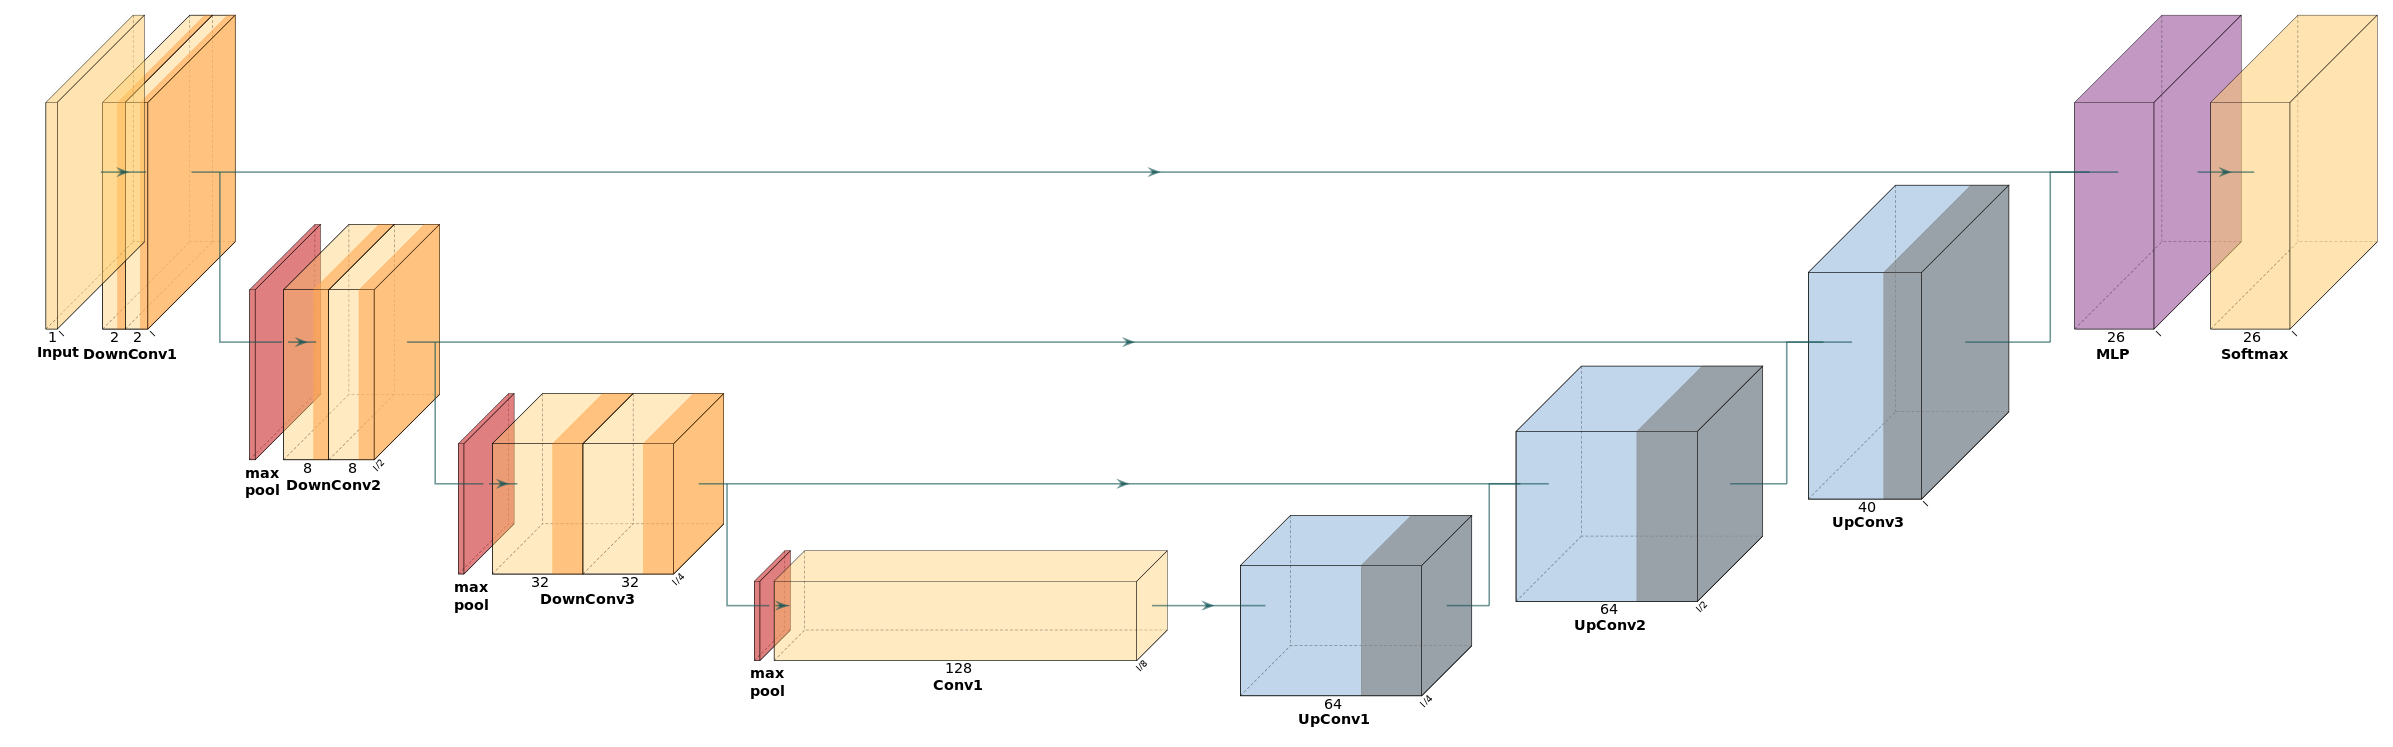
\includegraphics[width=\textwidth]{images/VUE_net_model.png}
  \caption{VUE-net architecture}
  \label{fig:model}
\end{figure*}

Given the similarity of our task with image encoding, we decided to take inspiration for our model architecture
from many different networks used for image segmentation. Our main inspiration was U-net \cite{Unet}.
This network exploits an autoencorder-like architecture to obtain the segmented image.
In particular, it uses convolution to extract features and maxpooling to downsample the image.
Another U-net element that inspired us is the use of concatenation in order to provide
residual connections between the "down" and "up" convolutions. It must be noted that
the authors of the paper used cropping in order to perform these operations, as the feature dimensions between layers do not exactly match. 
It will be shown later that our architecture does not suffer from this issue since we decided to simplify 
this process by having hidden states of equal size.
Another model architecture we took inspiration from was VoxSegNet \cite{VoxSegNet}. This architecture performs 
sequential extraction of features that are combined toghether, across different levels of extraction, to obtain a prediction. 
This is analogous to the residual but with some additional complexity that won't be
further explained in this paper. 
The specific VoxSegNet element we included in our model architecture is the use of convolutional layers with different dilation rates 
(atrous convolutions) in order to obtain features through kernels with different receptive fields.

Figure \ref{fig:model} illustrates the complete scheme of our model architecture, which is now going to be discussed.
For the down-convolution steps we used a custom \textit{DownConv} block that consists in two different
convolution layers, one with a dilation rate of 2 and a traditional one, which both double the number of features. 
The output of this layer is the concatenation of the results of the two convolutions.
Between steps, max pooling has been adopted to extract the more relevant features and to compress the representation.
At the "bottom" of the "convolutional ladder" a standard convolution that doubles the number of features has been used.
Then, each one of the up-convolution (also known as transposed convolution) steps is executed by a \textit{UpConv} block that halves the number of features
and increases the other dimensions, therefore expanding the data representation until layer \textit{UpConv3} matches the input dimensions.
As shown in the figure, this leads to a features number unbalance towards the ones coming from up-convolutions.
This was purposly done to give more importance to features of the new data representation that is expected to be more 
contiguos with respect to the original one that is affected by sparsity caused by the pointclouds sampling mentioned earlier.
In the end, a multi-layer perceptron (\textit{MLP}), made of two fully connected layers, has been used
to shrink the features dimensions to the number of classes (26) combined with a SoftMax layer that allows
to have the desired probability distribution.
Additionaly, between every subsequent convolutions Batch Normalization layers and ReLU activation functions were used.
This choice was made to stabilize the outputs of each layer and avoid overfitting. The ReLU in particular was chosen for
its general reliability and simplicity, as no particular properties were required
for the values of the in-between layers.

To obtain more accurate predictions, we created an additional ensemble-like model that exploits the previous
one robustness to input rotations which, as it will be explained later, is embedded at training time.
This network feeds the original model with the four possibile rotated versions of the given sample, 
aligns the received labels and returns their mean values.


\section{Training}
\begin{figure*}[ht]
    \centering
    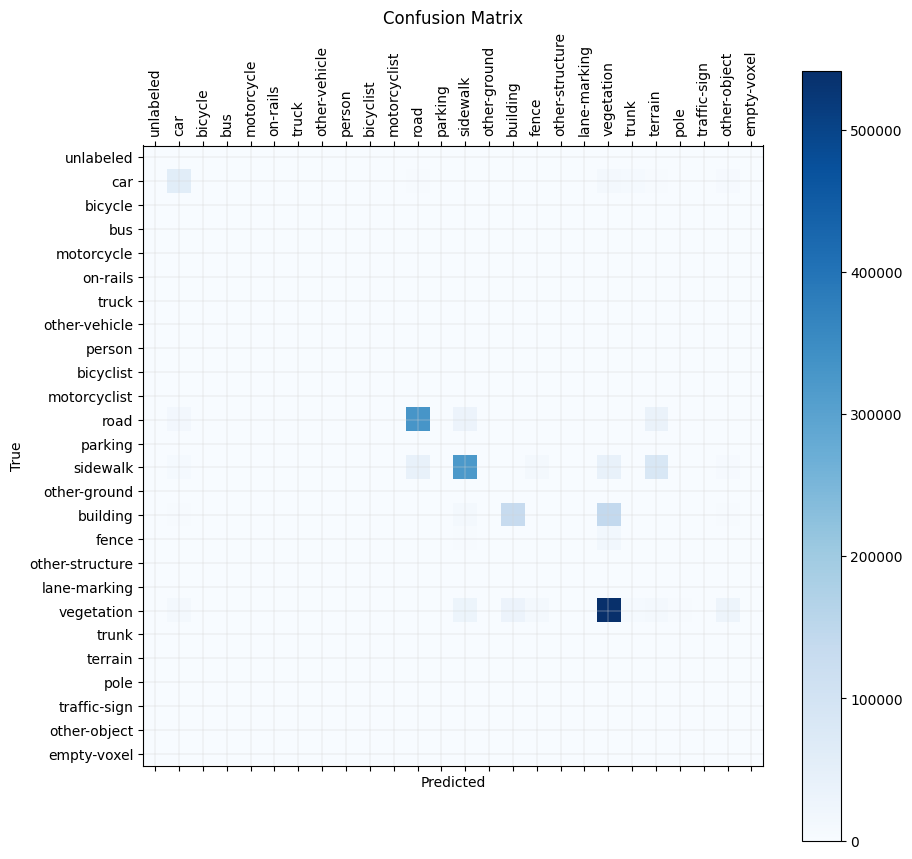
\includegraphics[width=0.5\textwidth]{images/confusion_matrix.png}
    \caption{Confusion matrix}
    \label{fig:matrix}
\end{figure*}

\begin{figure*}[ht]
    \centering
    \begin{subfigure}[b]{0.45\textwidth}
        \centering
        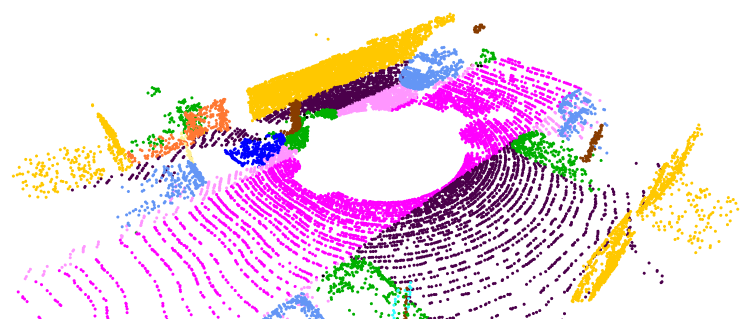
\includegraphics[width=\textwidth]{images/true.png}
        \caption{True labels}
        \label{fig:true}
    \end{subfigure}
    \hfill
    \begin{subfigure}[b]{0.45\textwidth}
        \centering
        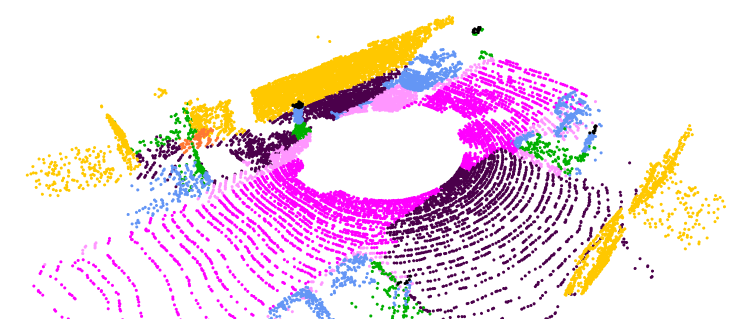
\includegraphics[width=\textwidth]{images/pred.png}
        \caption{Predicted labels}
        \label{fig:pred}
    \end{subfigure}
    \caption{True and predicted labels for pointcloud 55}
    \label{fig:visual}
\end{figure*}

The dataset made of 1000 sample was split into subsets of 750, 150 and 100 samples that correspond respectivly
to training, validation and test sets. In addition, samples from the training set were shuffled before being used.
The training phase was set such that for a determined number of epochs, the samples from the proper
set were loaded in batches of 10, rotated by 90 degrees around the z-axis by a random number
of times in the range 0-3 (to embedd robustness to such rotations in our model) and then given as 
input to the model, which performed the forward and backward propagation operations.
For this last operation, a loss function is needed.
We initially opted for the CrossEntropy loss, but we soon encountered poor results. This was due to the class imbalance of the
samples towards the "empty voxel" class. This happened for two reasons: first, by using voxelgrids instead of pointclouds
we introduced lots of empty space in our samples that had to be encoded too; second, the sampling of the pointclouds may lead 
to creating empty voxels that actually contain points.
We tried to address this issue by using the weighted version of CrossEntropy loss.
The weights were computed as as the inverse of the normalized sum of the class membership distribution probabilities 
over all voxels in the training set samples.
Even if this approach showed better performance, the class imbalance was too severe and the obtained results were not acceptable.
This lead us to our final choice for the loss function, Dice Loss.
This function allowed for fairly good model performance after training. This result is caused by the fact that Dice Loss considers 
the intersection over the union (IoU) of the predicted and true positive regions, which makes it particularly sensible to small 
and underrepresented classes.
After each epoch, validation was performed through the "ensamble" version of the model, introduced in the end of the last section,
to assess the current model performance and save it only if it was the best one seen so far. 
As for the Validation Loss we decided to use "one minus" the accuracy metric computed on the validation set samples.
This value is computed by a function that confronts each true and computed label tensors in their one-hot encoded version 
(argmax set to 1, others to 0) and returns the normalized count of pairs of different tensors.
By training our network for 50 epochs, we achieved a validation loss value of 0.280, which
means that it correcly labels 72.0\% of the samples voxels in the validation set.

\section{Performance}
Then, the test phase was performed. The test set used, composed by the last 100 samples, 
was not voxelized in order to test model performance on data in its original format.
To be able to achieve this, ad-hoc backpropagation functions were implemented.
Given a pointcloud, these functions attribute directly to each point the predicted label of the
corresponding voxel in the voxelized pointcloud (voxel grid).
With these operations, it was possibile to build the confusion matrix shown in figure \ref{fig:matrix}.
Using the data in this matrix, appropriate performance metrics were computed: Accuracy 0.691,
Precision 0.425, Recall 0.328 and F1-score 0.370.  

The first thing that can be noted is that only a few classes appear among test set pointclouds.
Secondly, it can be noted from the confusion matrix and guessed by the performance metrics, 
that our model is able to correctly classify the most popular classes such as \textit{car},
\textit{road}, \textit{sidewalk}, \textit{building} and \textit{vegetation} 
but lacks in performance for the others. 
However, the obtained results are still acceptable thanks to the great unbalance among point classes.

Using other Open3d functions, we were able to visualize the pointclouds with different colors depending
on their labels. Figure \ref{fig:visual} shows one of the pointclouds with the
correct colors (true labels) and the ones choosen by \textit{VUE-net} (predicted labels).
The observations made previously on performance agree with what can be seen from the images.
In fact, the model correcly predicts road, sidewalks, cars, buildings and vegetation but is not
able to recognize smaller, unpopular areas as the one in orange that corresponds to a fence.

\section{Results}
Using open3d functions we were able to visualize the pointclouds with different colors depending
on their labels. Figure \ref{fig:visual} shows a pointcloud with the
correct colors (true labels) and the one choosen by \textit{VUE-net} (predicted labels).
As it can be noted, the model easily recognizes streets, sidewalks, buildings and cars, 
which are the most frequent classes. Instead the underrepresented ones such as poles, vegetation
and fences are less precisely classified. To further improve \textit{VUE-net}, a way to
make the network pay even more attention to these classes must be found.

\nocite{*}
\newpage
\bibliography{aaai24}

\end{document}
